\section{Latency}\label{app:e2e}

Every replayed OBQA and ARC policy saves time, all of it on skipped queries, and every saving class holds in three repeats on a second hardware configuration (Figure~\ref{fig:savings}). Replays reuse the frozen thresholds and 128-question panels without recalibration, and all replayed outputs matched their development or same-replay fixed-reference counterparts (including every route and output of the medium-pair C2C replays), so only latency is re-measured (Table~\ref{tab:e2e_full}).

\begin{table}[!htbp]\centering\scriptsize
\caption{Every deployed Qwen-pair policy saves time on its OBQA or ARC panel and on the sealed ARC test; on MMLU-Pro only the Text saving is established. (a), (b): development replays on 128-question panels; (c): sealed test (1,172 questions); all on the first configuration. Saving: paired mean of fixed reference minus policy, every probe and cold request included [paired bootstrap 95\% CI]; not comparable across pairs or benchmarks. Cold request: a path's first request after model loading. $\Delta$acc: policy minus reference [paired bootstrap 95\% CI].}
\label{tab:e2e_full}
\setlength{\tabcolsep}{2pt}
\begin{tabular*}{\linewidth}{@{}l@{\hspace{6pt}}l@{\hspace{4pt}\extracolsep{\fill}}rcclccl@{}}\toprule
& & & \multicolumn{2}{c}{Mean latency (ms)} & & \multicolumn{2}{c}{Correct answers} & \\\cmidrule(lr){4-5}\cmidrule(lr){7-8}
Population & Reference & \multicolumn{1}{c}{Skipped} & Policy & Reference & \multicolumn{1}{c}{Saving (ms) [95\% CI]} & Policy & Reference & \multicolumn{1}{c@{}}{$\Delta$acc (points) [95\% CI]}\\\midrule
\multicolumn{9}{@{}l}{\emph{(a) Development end-to-end replay on 128-question panels, OBQA and ARC}}\\
medium/OBQA & C2C & 66/128 & 335.6 & 415.2 & 79.7 [48.1, 129.1] & 94 & 93 & $+0.78$ [0.00, $+2.34$]\\
medium/ARC & C2C & 77/128 & 352.4 & 453.1 & 100.7 [74.5, 133.1] & 85 & 85 & $+0.00$ [0.00, 0.00]\\
large/OBQA & Text & 97/128 & 505.1 & 1022.2 & 517.1 [447.8, 583.6] & 112 & 113 & $-0.78$ [$-3.91$, $+1.56$]\\
large/OBQA & C2C & 97/128 & 325.9 & 362.4 & 36.6 [18.0, 56.8] & 102 & 101 & $+0.78$ [0.00, $+2.34$]\\
large/ARC & Text & 120/128 & 372.7 & 1090.3 & 717.6 [670.6, 763.2] & 117 & 117 & $+0.00$ [$-2.34$, $+2.34$]\\
large/ARC & C2C & 115/128 & 329.9 & 440.8 & 110.9 [82.0, 142.8] & 115 & 114 & $+0.78$ [$-1.56$, $+3.91$]\\
\midrule
\multicolumn{9}{@{}l}{\emph{(b) Development replay, MMLU-Pro (same threshold and route set for both references)}}\\
large/MMLU-Pro & Text & 48/128 & 984.3 & 1330.7 & 346.3 [249.8, 443.0] & 65 & 63 & $+1.56$ [0.00, $+3.91$]\\
large/MMLU-Pro & C2C & 48/128 & 332.6 & 340.8 & 8.2 [$-20.5$, $+44.0$] & 55 & 55 & $+0.00$ [0.00, 0.00]\\
\midrule
\multicolumn{9}{@{}l}{\emph{(c) Sealed ARC-Challenge test}}\\
large/ARC & Text & 1100/1172 & 362.0 & 1047.7 & 685.6 [669.6, 700.8] & 1080 & 1085 & $-0.43$ [$-1.19$, $+0.26$]\\
large/ARC & C2C & 1047/1172 & 323.6 & 414.5 & 90.9 [81.0, 101.0] & 1061 & 1057 & $+0.34$ [$-0.17$, $+0.85$]\\
\bottomrule\end{tabular*}
\end{table}


\paragraph{Per-request distribution.} The policy's 99th-percentile latency is never above the reference's in any replay; its 90th percentile is above it only for medium/OBQA/C2C and, on the second configuration, large/MMLU-Pro/Text. Routed queries are slower in 84.6 to 100\% of cases (median $-25$ to $-45$~ms, the probe cost), meaning the entire saving stems from skipped queries (also under argmax answering), and the paired median is negative in 16 of 58 arm-streams. The probe costs 32.88 and 43.37~ms on the small- and large-pair OBQA panels, of which the prefill with its last-position projection takes 31.25 and 41.79~ms (95 to 96\%), and 48.4 and 46.1~ms on the MMLU-Pro replay, whose paired median savings are $-41.3$ and $-43.6$~ms (median latencies 1170.6 vs.\ 1273.1~ms for Text, and 293.6 vs.\ 250.9~ms for C2C). The probe, vendor runner, and official fuser are single-row, so no batched comparison is reported.

\paragraph{Component estimates and complete replays.} Before any replay, each policy's cost was recomposed from timed components (the probe's stages plus the selected historical action request), without cache or prefill discounts. For the four large-pair policies, the complete replay saved 1.76~ms less than this estimate for OBQA/Text and 8.40, 20.50, and 9.74~ms more for OBQA/C2C, ARC/Text, and ARC/C2C (Figure~\ref{fig:savings}). A CPU recombination of development timings had projected 68.3 and 105.4~ms for the medium pair, whose replays saved 79.7 and 100.7~ms (median latencies 334.6 vs.\ 388.2~ms on OBQA, and 287.8 vs.\ 412.4~ms on ARC; paired median savings 79.3 and 81.6~ms).

\begin{figure}[!t]\centering
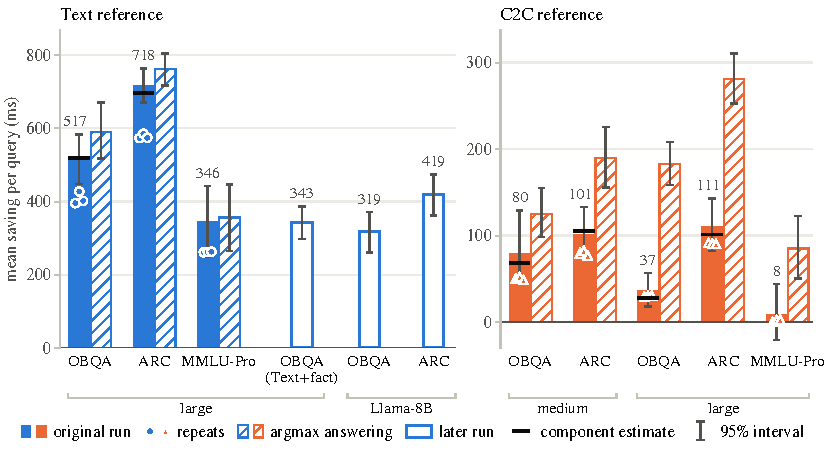
\includegraphics[width=\linewidth]{figures/figure_savings.pdf}
\caption{Every saving class holds across configurations, repeats, and probe-cache reuse (under argmax answering, large/MMLU-Pro/C2C's interval moves above zero), and the component estimates fixed before the replays are close to the complete replays. Mean saving per query of each replayed policy, Text-reference policies left and C2C-reference policies right (separate scales), with paired bootstrap 95\% intervals as whiskers: solid bar, the original run (first configuration; Table~\ref{tab:e2e_full}), its mean printed above; markers on it, the means of the three repeats on the second configuration (Table~\ref{tab:repeats}); outlined bar, the single later run of Text+fact or a Llama-8B policy on the second configuration (Table~\ref{tab:u0saving}); hatched bar, answering skipped questions from the probe's argmax (second configuration; Table~\ref{tab:impl}); black tick, the component estimate (large-pair OBQA and ARC; from timed probe stages and historical action requests) or CPU recombination (medium pair; from development timings) fixed before the replays. Saving class: interval above, below, or including zero. Savings from the two configurations are not comparable in absolute terms; only large/MMLU-Pro/C2C has an interval containing zero, in every original and repeat run.}
\label{fig:savings}
\end{figure}

\paragraph{Busy GPU time.} Under rules fixed before computing, busy GPU time (summed wall time of GPU-side stages on both GPUs) can be computed only for replays timing each stage separately; thus, it is available for four of the eight policies (large-pair OBQA and ARC replays), where the busy-time saving accounts for 88 to 99\% of the latency saving (Table~\ref{tab:busy}).

\begin{table}[!htbp]\centering\scriptsize
\caption{Busy GPU time saved is 88 to 99\% of the latency saved on the four large-pair panels. Original runs (first configuration). Busy GPU time: summed wall time of GPU-side stages on both GPUs. Intervals: paired bootstrap 95\% CI.}
\label{tab:busy}
\setlength{\tabcolsep}{2pt}
\begin{tabular*}{\linewidth}{@{}l@{\hspace{6pt}}l@{\hspace{6pt}}l@{\hspace{4pt}\extracolsep{\fill}}cccc@{}}\toprule
& & & \multicolumn{3}{c}{Saving (ms) [95\% CI]} & \\\cmidrule(lr){4-6}
Pair & Task & Reference & Busy GPU time & Latency & Busy minus latency & \multicolumn{1}{c@{}}{Busy / latency}\\\midrule
large & OBQA & Text & 513.5 [448.7, 574.2] & 517.1 [447.8, 583.6] & $-3.6$ [$-9.9$, $+8.3$] & 0.993\\
large & OBQA & C2C & 32.3 [14.4, 51.8] & 36.6 [18.0, 56.8] & $-4.3$ [$-6.3$, $-3.2$] & 0.882\\
large & ARC & Text & 705.2 [659.1, 750.0] & 717.6 [670.6, 763.2] & $-12.4$ [$-13.2$, $-11.6$] & 0.983\\
large & ARC & C2C & 106.6 [77.8, 138.2] & 110.9 [82.0, 142.8] & $-4.3$ [$-4.6$, $-3.9$] & 0.961\\\bottomrule
\end{tabular*}
\end{table}

\paragraph{Second configuration and port check.}\label{app:revision} Repeats and variants, added after main results under protocols fixed before outcomes, ran on exclusively allocated nodes with four A100-SXM4-40GB GPUs connected via NVLink (two used with the original placement, while original runs used two of eight A100-SXM4-40GB GPUs on a shared node). The repeats followed bit-for-bit reproduction of saved outputs: the receiver-only outputs of all seven development populations, large-pair ARC receiver-only and C2C outputs, and learned predictor features and predictions. In a post-hoc port check, our runtime and the official C2C evaluator \citep{fu2025c2c}, using byte-identical prompts, produce identical raw outputs on all 500 official OBQA test questions for every pair and action. Small-pair C2C answers 263/500 correctly, matching published results, whereas medium and large C2C answer fewer correctly than $R$ under our parser (317 vs.\ 327 and 405 vs.\ 425) and official scoring (321 vs.\ 326 and 395 vs.\ 425; small pair: 263 vs.\ 198). The published main evaluation uses Qwen3-0.6B as its only receiver, and the authors' scaling study uses several Qwen3 receivers with fusers trained on MMLU's auxiliary training split and reports smaller relative gains for larger receivers \citep{fu2025c2c}, so no published accuracy exists for released general-purpose medium and large fusers; for those pairs, byte-identical outputs serve as the relevant check.

\paragraph{Repeated replays.} Under a rule fixed before any repeat, each of the eight replays ran three additional times on the second configuration, maintaining frozen thresholds, panels, arm rotation, and the timing boundary. The rule defines a policy's class on savings excluding questions where either arm made its first request after model loading (Table~\ref{tab:repeats}b): \checkmark\ if the interval lies above zero, $\times$ if below, and ? otherwise. Original classes had to be reproduced by all eight policies across all three repeats, which they were; the classes are the same over all requests (Table~\ref{tab:repeats}a). Online scores, inputs, and routes matched frozen records in every repeat, and every output matched its development or same-run counterpart. Absolute savings differ across configurations and are not comparable; large/MMLU-Pro/Text saves 261.4 to 263.5~ms there, and MMLU-Pro paired medians are negative ($-21$ to $-41$~ms; $-21$ to $-32$~ms for Text), mirroring the original panel.

\begin{table}[!htbp]\centering\scriptsize
\caption{Every replayed policy keeps its prespecified saving class in all three repeats. Paired mean saving (ms) [95\% CI]. Saving class: all four intervals of the row lie above zero (\checkmark) or all include zero (?). Cold first request: a path's first request after model loading. Configurations are not comparable.}
\label{tab:repeats}
\setlength{\tabcolsep}{1pt}
\begin{tabular*}{\linewidth}{@{}l@{\hspace{3pt}\extracolsep{\fill}}llccccl@{}}\toprule
& & & First configuration & \multicolumn{3}{c}{Second configuration} & \\\cmidrule(lr){4-4}\cmidrule(lr){5-7}
Pair & Task & Reference & Original run & Repeat 1 & Repeat 2 & Repeat 3 & Saving class\\\midrule
\multicolumn{8}{l}{\emph{(a) All requests}}\\
large & OBQA & Text & 517.1 [447.8, 583.6] & 395.5 [325.3, 458.3] & 427.6 [376.4, 474.4] & 401.8 [335.6, 460.6] & \checkmark\ above 0\\
large & OBQA & C2C & 36.6 [18.0, 56.8] & 29.4 [14.9, 45.5] & 30.3 [15.7, 46.5] & 30.4 [15.5, 46.6] & \checkmark\ above 0\\
large & ARC & Text & 717.6 [670.6, 763.2] & 573.5 [536.0, 608.7] & 585.4 [546.7, 622.9] & 574.2 [536.3, 611.2] & \checkmark\ above 0\\
large & ARC & C2C & 110.9 [82.0, 142.8] & 91.4 [68.9, 116.2] & 90.5 [67.3, 115.4] & 90.2 [66.9, 115.8] & \checkmark\ above 0\\
medium & OBQA & C2C & 79.7 [48.1, 129.1] & 49.9 [35.8, 65.5] & 52.2 [37.7, 67.9] & 48.5 [34.3, 64.4] & \checkmark\ above 0\\
medium & ARC & C2C & 100.7 [74.5, 133.1] & 79.2 [58.5, 104.5] & 82.4 [61.4, 108.4] & 76.5 [56.5, 101.2] & \checkmark\ above 0\\
large & MMLU-Pro & Text & 346.3 [249.8, 443.0] & 261.4 [191.1, 331.5] & 262.4 [192.3, 331.1] & 263.5 [193.5, 333.7] & \checkmark\ above 0\\
large & MMLU-Pro & C2C & 8.2 [$-20.5$, $+44.0$] & $-0.1$ [$-23.4$, $+27.8$] & 2.4 [$-20.3$, $+30.6$] & 2.6 [$-20.1$, $+30.4$] & ? includes 0\\\midrule
\multicolumn{8}{l}{\emph{(b) Questions with a cold first request excluded ($N=127$); the class rule uses these}}\\
large & OBQA & Text & 532.8 [470.9, 594.7] & 419.6 [370.7, 468.7] & 430.2 [380.9, 479.9] & 423.1 [373.6, 471.5] & \checkmark\ above 0\\
large & OBQA & C2C & 33.5 [16.5, 51.7] & 27.4 [13.8, 42.3] & 29.3 [14.9, 44.2] & 27.8 [13.9, 42.5] & \checkmark\ above 0\\
large & ARC & Text & 717.2 [670.1, 761.8] & 573.2 [535.8, 609.6] & 585.0 [547.0, 621.8] & 573.8 [535.2, 610.6] & \checkmark\ above 0\\
large & ARC & C2C & 112.3 [83.7, 142.3] & 92.4 [70.2, 115.8] & 91.6 [68.5, 115.7] & 91.2 [68.9, 115.1] & \checkmark\ above 0\\
medium & OBQA & C2C & 61.0 [43.9, 79.9] & 47.3 [34.0, 61.9] & 50.0 [36.4, 65.2] & 45.6 [32.5, 60.1] & \checkmark\ above 0\\
medium & ARC & C2C & 100.8 [73.0, 132.8] & 79.3 [57.6, 104.3] & 82.5 [60.1, 108.4] & 76.6 [55.4, 101.1] & \checkmark\ above 0\\
large & MMLU-Pro & Text & 322.1 [234.8, 412.5] & 260.8 [189.9, 333.9] & 261.0 [189.7, 335.1] & 262.7 [191.1, 336.5] & \checkmark\ above 0\\
large & MMLU-Pro & C2C & 6.5 [$-23.3$, $+41.1$] & $-0.0$ [$-24.5$, $+28.3$] & 2.6 [$-21.1$, $+30.5$] & 2.8 [$-20.7$, $+30.8$] & ? includes 0\\\bottomrule
\end{tabular*}
\end{table}

\begin{table}[!htbp]\centering\scriptsize
\caption{Answering skipped questions from the probe's argmax raises every saving, whereas reusing the probe's cache changes none by more than 5~ms (one run on the second configuration; paired mean saving, ms [95\% CI]). Original: receiver rerun after the probe.}
\label{tab:impl}
\setlength{\tabcolsep}{2pt}
\begin{tabular*}{\linewidth}{@{}l@{\hspace{6pt}}l@{\hspace{6pt}}l@{\hspace{4pt}\extracolsep{\fill}}rrr@{}}\toprule
& & & \multicolumn{3}{c@{}}{Paired mean saving (ms) [95\% CI]}\\\cmidrule(l){4-6}
Pair & Task & Reference & \multicolumn{1}{c}{Original} & \multicolumn{1}{c}{Reuse} & \multicolumn{1}{c@{}}{Argmax}\\\midrule
large & OBQA & Text & 436.3 [378.6, 503.2] & 437.8 [378.1, 506.0] & 589.7 [518.0, 670.3]\\
large & OBQA & C2C & 31.2 [16.7, 47.3] & 31.0 [16.5, 47.0] & 182.9 [158.2, 208.1]\\
large & ARC & Text & 565.6 [528.6, 601.4] & 564.4 [527.5, 599.6] & 762.7 [717.4, 804.3]\\
large & ARC & C2C & 91.9 [69.5, 116.6] & 90.5 [68.3, 115.0] & 280.8 [252.7, 310.4]\\
medium & OBQA & C2C & 50.1 [36.0, 65.6] & 49.9 [35.7, 65.6] & 125.2 [98.3, 154.9]\\
medium & ARC & C2C & 77.9 [57.4, 103.0] & 78.2 [57.5, 103.5] & 189.5 [155.4, 225.4]\\
large & MMLU-Pro & Text & 275.2 [199.6, 348.5] & 280.0 [203.5, 354.2] & 356.5 [265.1, 446.7]\\
large & MMLU-Pro & C2C & 4.6 [$-18.0$, $+32.6$] & 6.9 [$-15.8$, $+35.4$] & 85.0 [50.3, 122.8]\\\bottomrule
\end{tabular*}
\end{table}

\paragraph{Cheaper implementations.} Our replays rerun the receiver after the probe. In an additional run (protocol fixed before any output), four arms were interleaved per policy: the fixed reference, the original policy, a \emph{reuse} policy continuing the receiver-only answer from the probe's KV cache (the receiver prompt is an exact token prefix of the probe input), and an \emph{argmax} policy answering skipped questions from the probe's argmax without sending a receiver request. Argmax labels match native receiver answers on 88 to 100\% of calibration questions, and recertifying with them retains every threshold except medium/OBQA/C2C ($q=0.50$). Argmax answering boosts every saving, for instance MMLU-Pro C2C from 4.6 to 85.0~ms [50.3, 122.8], and narrows the Text-to-C2C saving ratio from 14.0 and 6.2 to 3.2 and 2.7 on OBQA and ARC (4.2 on MMLU-Pro). Its paired medians are negative on MMLU-Pro and medium/OBQA/C2C because gains concentrate on the skipped minority. Reuse alters no saving by more than 5~ms (Table~\ref{tab:impl}): it skips only the receiver's prefill of its own prompt, which changes a skipped request's action time by between 0.4~ms more and 6.3~ms less, while the probe is still paid on every query. Reuse outputs differed from native outputs on 13 of 668 skipped requests (exclusively via trailing periods or extended probe answer phrases) and never in parsed labels.

\begin{table}[!htbp]\centering\scriptsize
\caption{Only the two large MMLU-Pro policies are flagged by the prespecified rule (coverage off by more than 10 points (0.10) or an absolute length SMD (standardized mean difference) above 0.2). Population: all development questions. Eq.~\eqref{eq:saving} saving (ms) with the panel's latencies (first configuration; Text+fact and Llama-8B: second) and the panel's or the population's coverage.}
\label{tab:panelrep}
\renewcommand{\arraystretch}{1.1}\setlength{\tabcolsep}{3pt}
\begin{tabular*}{\linewidth}{@{}l@{\hspace{5pt}\extracolsep{\fill}}cccccc@{}}\toprule
& \multicolumn{2}{c}{Coverage} & \multicolumn{2}{c}{Largest $|$SMD$|$} & \multicolumn{2}{c}{Eq.~\eqref{eq:saving} saving (ms) with}\\\cmidrule(lr){2-3}\cmidrule(lr){4-5}\cmidrule(l){6-7}
Policy & panel & population & value & feature & panel coverage & population coverage\\\midrule
large/OBQA/Text & 0.758 & 0.771 & 0.136 & helper message & 517.2 & 527.1\\
large/OBQA/C2C & 0.758 & 0.771 & 0.115 & reference output & 36.6 & 38.0\\
large/ARC/Text & 0.938 & 0.950 & 0.053 & question & 717.8 & 727.8\\
large/ARC/C2C & 0.898 & 0.903 & 0.057 & reference output & 110.9 & 111.7\\
large/MMLU-Pro/Text & 0.375 & 0.405 & 0.212 & receiver output & 317.0 & 346.0\\
large/MMLU-Pro/C2C & 0.375 & 0.405 & 0.212 & receiver output & 5.6 & 9.7\\
medium/OBQA/C2C ($q=0.55$) & 0.516 & 0.526 & 0.107 & receiver output & 56.8 & 58.6\\
medium/ARC/C2C & 0.602 & 0.632 & 0.053 & question & 100.6 & 107.4\\
large/OBQA/Text+fact & 0.719 & 0.722 & 0.123 & helper message & 339.5 & 341.4\\
Llama-8B/OBQA/Text & 0.594 & 0.590 & 0.136 & helper message & 322.4 & 320.3\\
Llama-8B/ARC/Text & 0.688 & 0.689 & 0.069 & receiver output & 417.2 & 418.2\\\bottomrule
\end{tabular*}
\end{table}

\paragraph{Full MMLU-Pro population and panel representativeness.} Across all 2,641 MMLU-Pro development questions, the C2C policy saves a mean of 23.3~ms [14.5, 32.2] on the second configuration (22.0~ms [14.0, 30.5] excluding the single cold question; paired median $-37.3$~ms), an order of magnitude below the Text panel saving on that configuration. Under rules fixed before computing, each panel was compared with its full development population across question, message, and output lengths, share of $u=0$ questions, and coverage, flagging policies whose coverage differs by over 10 points or whose length SMD exceeds 0.2. Only the two large MMLU-Pro policies are flagged due to slightly longer receiver-only outputs (5.70 vs.\ 5.54 tokens; SMD 0.212) and 3.0 points lower coverage (Table~\ref{tab:panelrep}). Applying population coverage to Eq.~\eqref{eq:saving} alters the saving by 0.8 to 29.0~ms; C2C saves only 5.6~ms (9.7~ms with population coverage). The 128 panel questions of the full MMLU-Pro C2C replay save 4.5~ms, versus 23.3~ms across all 2,641 questions (SMD $-0.08$).

\paragraph{Later replays and costs.} A Text-only replay driver copy (22 changed lines, including two-arm rotation; an approved deviation) reproducing 16 saved rows byte for byte measured Llama-8B savings of 318.6~ms [261.1, 372.1] and 418.9~ms [361.7, 473.7] on the second configuration (fixed Text 770.3 and 818.4~ms, policy 451.7 and 399.5~ms; 325.5 and 417.6~ms excluding the first request), though 39 and 27\% of queries run slower since queries keeping Text also pay the probe. There, the Text+fact policy skips 92 of 128 panel questions, changes 5, reduces mean latency from 726.5 to 383.1~ms, a saving of 343.4~ms [297.7, 386.0] (paired median 448.5~ms), and answers 116 panel questions correctly vs.\ 121 for reference. Standalone calibration requires $2N_{\rm cal}$ machine requests ($3N_{\rm cal}$ comparing both references with shared $R$). Using mean savings from the second configuration, if reference outputs come from served traffic, fit and calibration requests amortize after 230 (large/ARC/Text) to 76,205 queries (large/MMLU-Pro/C2C), within 6,415 queries for every Text reference, and after 905 to 152,171 queries if references must also run. A small-LLM controller branch (small helper producing communicate-or-skip probabilities) halted at a predetermined cost screen: the controller alone took 21.6~ms (54.5~ms with probe), and even the fastest controller plus probe (51.7~ms) exceeded an optimistic 43.0~ms saving bound, precluding signal evaluation.
